\documentclass{article}
\usepackage{graphicx}
\usepackage{amsmath}
\graphicspath{ {./pictures/} }

\title{Pixel}
\author{Maciej Maj}
\date{\today}

\begin{document}
\maketitle
\section{Wstęp}
Przykład wyrażenia matematycznego:
\begin{equation}
    (a+b)^2=a^2+2ab+b^2
\end{equation}
Przykładowe zdjęcie:
\begin{figure}[h]
    \centering
    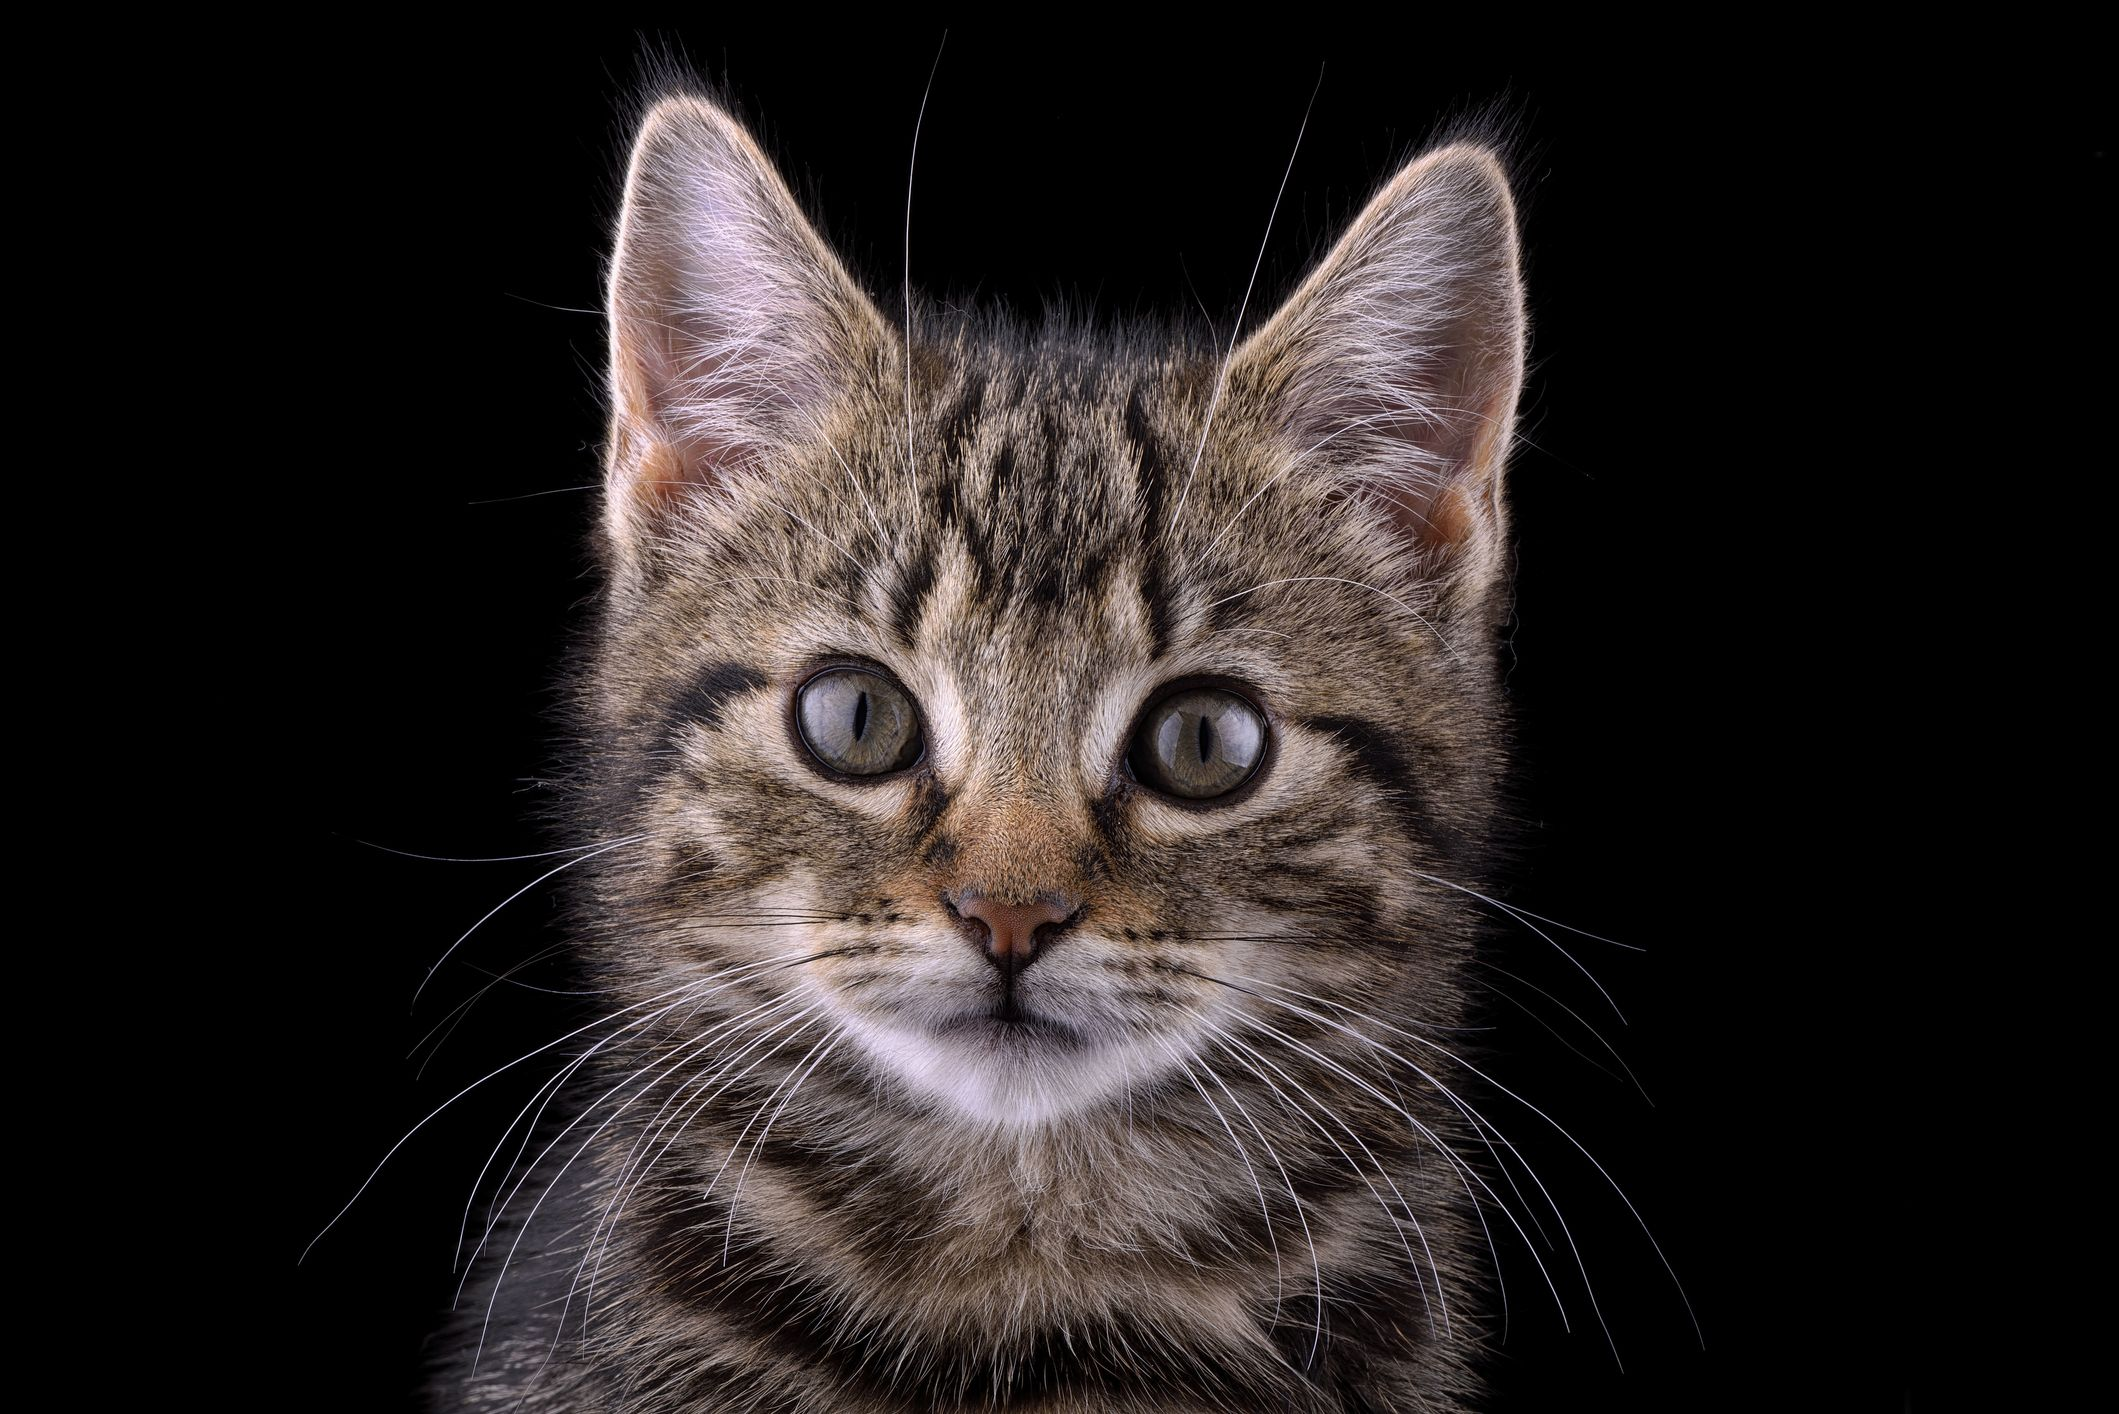
\includegraphics[width=0.4\textwidth]{pictures/fota.jpg}
    \caption{Mamy tu piekny okaz kota}
    \label{fig:kot}
\end{figure}
\section{Tabela}\label{sec:tabela}
\begin{table}[h]
    \centering
    \begin{tabular}{|a|a|a|}
        \hline
        Zwierzęta & Ludzie & Zarobki
        \\
        \hline
        Kot & Tomek & 1100zł \\
        Pies & Piotr & 2100zł \\ 
        Rybki & Jakub & 1700zł \\
        \hline
        \end{tabular}
        \caption{Tabela 1}
    \end{table}
\section{Listy}\label{sec:listy}
To jest lista numerowana
\begin{enumerate}
    \item Język C
    \item Język C++
    \item Python
\end{enumerate}
To jest lista nienumerowana
\begin{itemize}
    \item program 1
    \item program 2
    \item program 3
\end{itemize}

\textbf{Kot domowy} - udomowiony gatunek ssaka z rzędu drapieżnych \emp{z rodziny kotowatych}. Koty zostały udomowione około 9500 lat temu i są obecnie najpopularniejszymi zwierzętami domowymi na świecie. W sekcji \ref{sec:listy} znajduje się przykładowa lista, a w sekcji \ref{sec:tabela} jest tabela, 

\end{document}